\documentclass[handout]{beamer}
\usepackage{graphicx}
\usepackage{caption}
\usepackage{subcaption}
\graphicspath{ {./img/} }
\usetheme{default}

\title{Molecular dynamics study of ideal polymer chains with variable persistence length}
\subtitle{Short progress report}
\author{Yahor Paromau, Holger Merlitz}
\institute{ITP@IPF}
\date{23.05.2023}

\newcommand{\mean}[1]{\langle #1 \rangle}

\begin{document}


\begin{frame}
    \titlepage
\end{frame}


\begin{frame}
    \frametitle{Outline}
    \tableofcontents
\end{frame}

\section{Introduction}

\begin{frame}
    \frametitle{Definitions, notations, units}
    Mostly: following \cite{svaneborg_2020}

    Units: LJ

    Notations and definitions:

    \begin{itemize}
        \item Contour length: $L$
        \item End to End distance (ETE): $\vec{R}$
        \item Change of ETE: $[\Delta R(t)]^2 := [\vec{R}(t)-\vec{R}(0)]^2$
        \item Friction coefficient of bead, viscosity: $\zeta$ $[\frac{\textrm{mass}}{\textrm{time}}]$, $\eta$ $[\frac{\textrm{mass}}{\textrm{time} * \textrm{distance}}]$
        \item subscript "$b$" to denote bead specific properties to distinguish these from Kuhn units:
            \begin{itemize}
                \item Kuhn lenght, bond length: $l_K$, $l_b$
                \item Number of Kuhn segments, number of beads: $N_K$, $N_b$
            \end{itemize}
        \item Friction coefficient of center of mass: $\zeta_{CM}=N_b \zeta$ 
        \item Rouse relaxation time \cite{svaneborg_2020}: $\tau_R = \frac{1}{3 \pi^2} \frac{\zeta_{CM} \mean{R^2}}{k_B T} = \frac{1}{3 \pi^2} \frac{\zeta N_b^2 l_b^2}{k_B T}$
        \item Relaxation time of single bead: $\tau_0 = \frac{3\pi^2 \tau_R}{N^2}$ 
    \end{itemize}

\end{frame}
    

\begin{frame}
    \frametitle{Assumptions}
    \begin{itemize}
        \item Variation of $0.2\%$ of $l_b$ is neglectible \cite{svaneborg_2020} 
        
        $\Rightarrow$ $l_b=const$, $L=(N_b-1) l_b$=const

        \item ...
    \end{itemize} 
\end{frame}


\begin{frame}
    \frametitle{Rouse model}
    \begin{equation}
        \mean{R^2}=N_b l_b^2
    \end{equation}
    \begin{equation}
        g_4(t) := \mean{(\Delta R(t))^2} = 2 N_b l_b^2 (1-\frac{8}{\pi^2}\sum_{p=1,3,...}e^{\frac{-t p^2}{\tau_R}})
    \end{equation}

\end{frame}

\section{Experiment 1: Fully flexible chain}


\begin{frame}
    \frametitle{Experiment 1: Fully flexible chain}
    \framesubtitle{Settings}
    Same potentials used as in \cite[Section 2.1]{svaneborg_2020}, except:
    \begin{itemize}
        \item Bending potential: $U_{bend}(\theta)=0$
        \item Only bonded beads interract
    \end{itemize}
\end{frame}


\begin{frame}
    \frametitle{Experiment 1: Fully flexible chain}
    \framesubtitle{$\tau_R$ calculated analytically}

    \begin{figure}[h]
        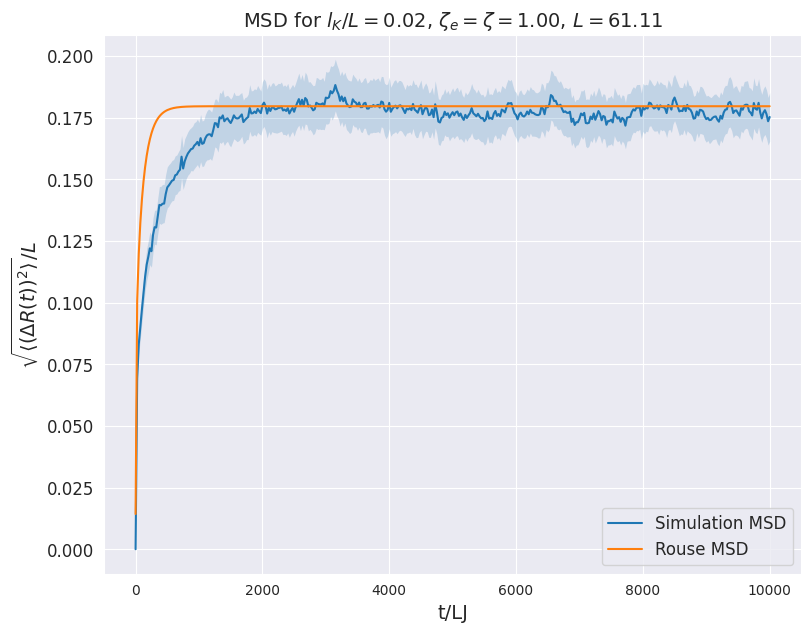
\includegraphics[width=9.5cm]{./3-exp-fixed-param.png}
    \end{figure}
\end{frame}


\begin{frame}
    \frametitle{Experiment 1: Fully flexible chain}
    \framesubtitle{$\tau_R$ as free parameter}

    \begin{figure}[h]
        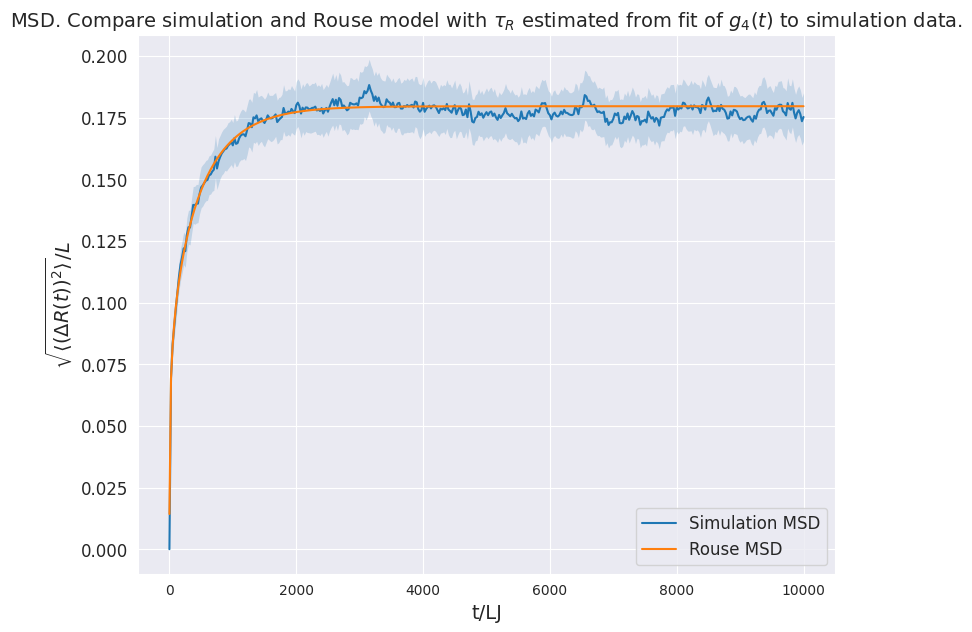
\includegraphics[width=10.8cm]{./3-exp-free-param.png}
    \end{figure}
\end{frame}


\begin{frame}
    \frametitle{Experiment 1: Fully flexible chain}
    \framesubtitle{$\tau_R$ analytcal/free values}

    Analytical: $\tau_R=520.64$, $\tau_0=0.032$
    \\
    Free parameter: $\tau_R=2136.5 \pm 155.2$, $\tau_0=0.130 \pm 0.009$
    \\
    \vspace{1cm}
    Define adjustment factor
    $ \alpha := \frac{\tau_{0, \textrm{empirical}}}{\tau_{0, \textrm{analytical}}} \approx 4.047$
\end{frame}

\section{Experiment 2: Semi-flexible chain, vary persistence length}

\begin{frame}
    \frametitle{Experiment 2: Semi-flexible chain, vary persistence length}
    \framesubtitle{Settings}
    Same potentials used as in \cite[Section 2.1]{svaneborg_2020}, except:
    \begin{itemize}
        \item Only bonded beads interract
    \end{itemize}
\end{frame}

\begin{frame}
    \frametitle{Experiment 2: Semi-flexible chain, vary persistence length}
    \framesubtitle{Used equations}

    Kuhn length \cite{svaneborg_2020}:
    \begin{equation}
        l_K = l_b \frac{2\kappa + e^{-2 \kappa} - 1}{1-e^{-2\kappa}(2 \kappa + 1)}
    \end{equation}
    Number of Kuhn segments:
    \begin{equation} 
        N_K = \frac{L}{l_K}
    \end{equation}
    Rouse time:
    \begin{equation} \label{eq:tau_R_kuhn}
        \tau_R = \frac{1}{3 \pi^2} \frac{\zeta_{K} \mean{R^2}}{k_B T} = \frac{1}{3 \pi^2} \frac{\zeta N_b N_K l_K^2}{k_B T}
    \end{equation}
\end{frame}


\begin{frame}
    \frametitle{Experiment 2: Semi-flexible chain, vary persistence length}
    \framesubtitle{ETE in equilibrium}

    \begin{figure}[h]
        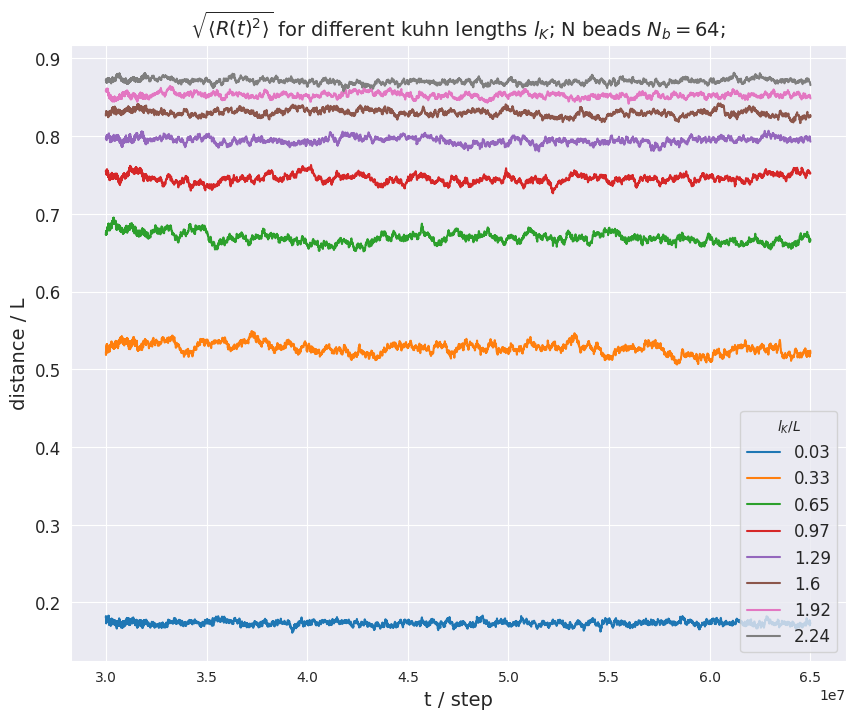
\includegraphics[width=8cm]{./4-exp-R_equi.png}
    \end{figure}
\end{frame}


\begin{frame}
    \frametitle{Experiment 2: Semi-flexible chain, vary persistence length}
    \framesubtitle{ETE vs Kuhn length}

    \begin{figure}[h]
        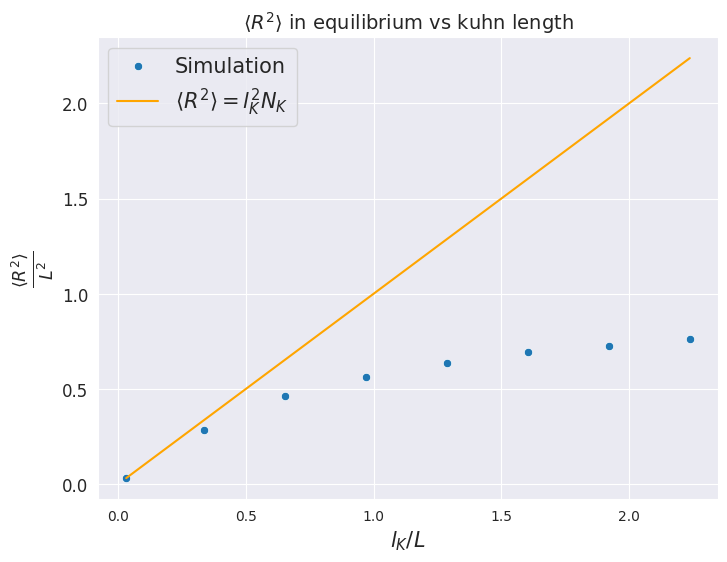
\includegraphics[width=8cm]{./4-exp-R_sim_vs_theor.png}
    \end{figure}
\end{frame}


\begin{frame}
    \frametitle{Experiment 2: Semi-flexible chain, vary persistence length}
    \framesubtitle{MSD: $\mean{[\Delta R(t)]^2}$}

    \begin{figure}[h]
        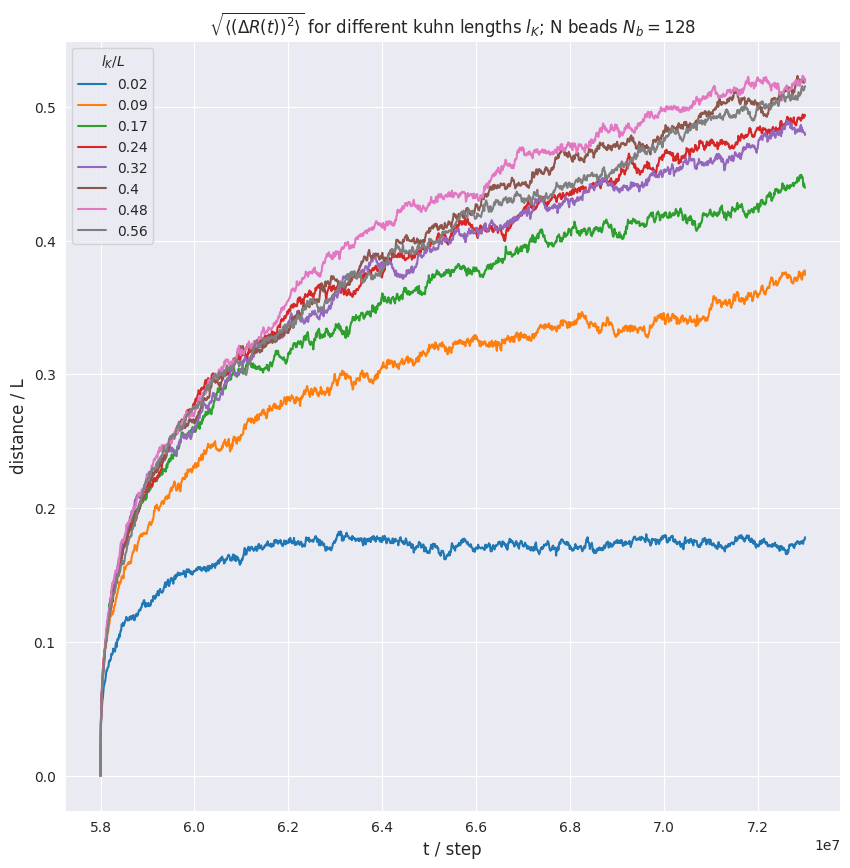
\includegraphics[width=9.5cm]{./4-exp-delta_R-bare.png}
    \end{figure}
\end{frame}

\begin{frame}
    \frametitle{Experiment 2: Semi-flexible chain, vary persistence length}
    \framesubtitle{MSD: $\mean{[\Delta R(t)]^2}$ on log-log scale}

    \begin{figure}[h]
        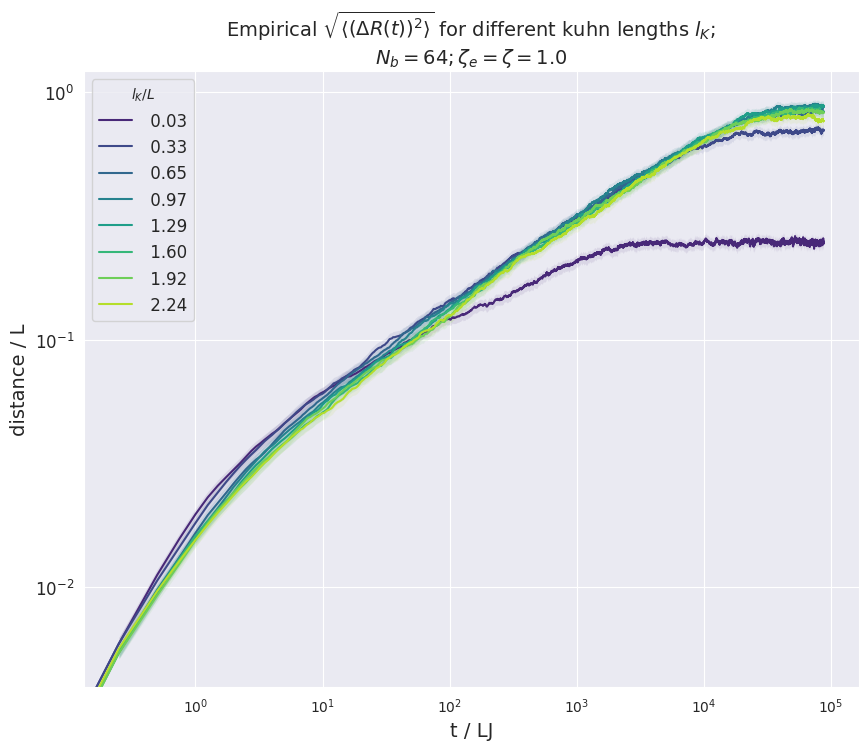
\includegraphics[width=9.5cm]{./4-exp-msd-log.png}
    \end{figure}
\end{frame}

\begin{frame}
    \frametitle{Experiment 2: Semi-flexible chain, vary persistence length}
    \framesubtitle{MSD: $\mean{[\Delta R(t)]^2}$ by dimension}

    \begin{figure}[h]
        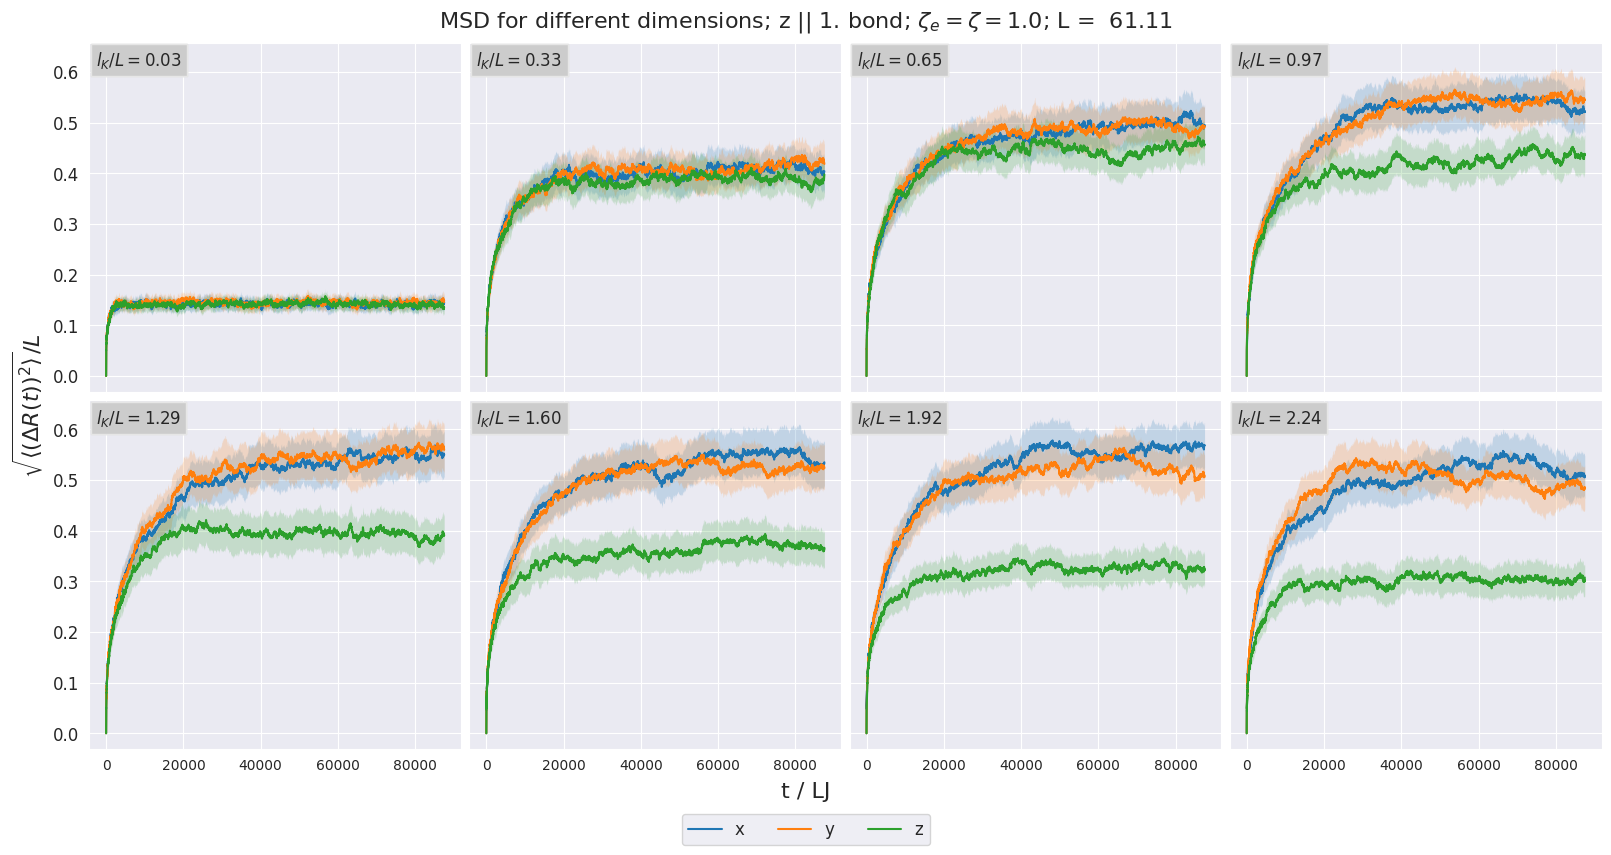
\includegraphics[width=11cm]{./4-exp-msd_by_dim.png}
    \end{figure}
\end{frame}



\begin{frame}
    \frametitle{Experiment 2: Semi-flexible chain, vary persistence length}
    \framesubtitle{$\mean{[\Delta R(t)]^2}$ vs Rouse with $\tau_R$ analytically}

    \begin{figure}[h]
        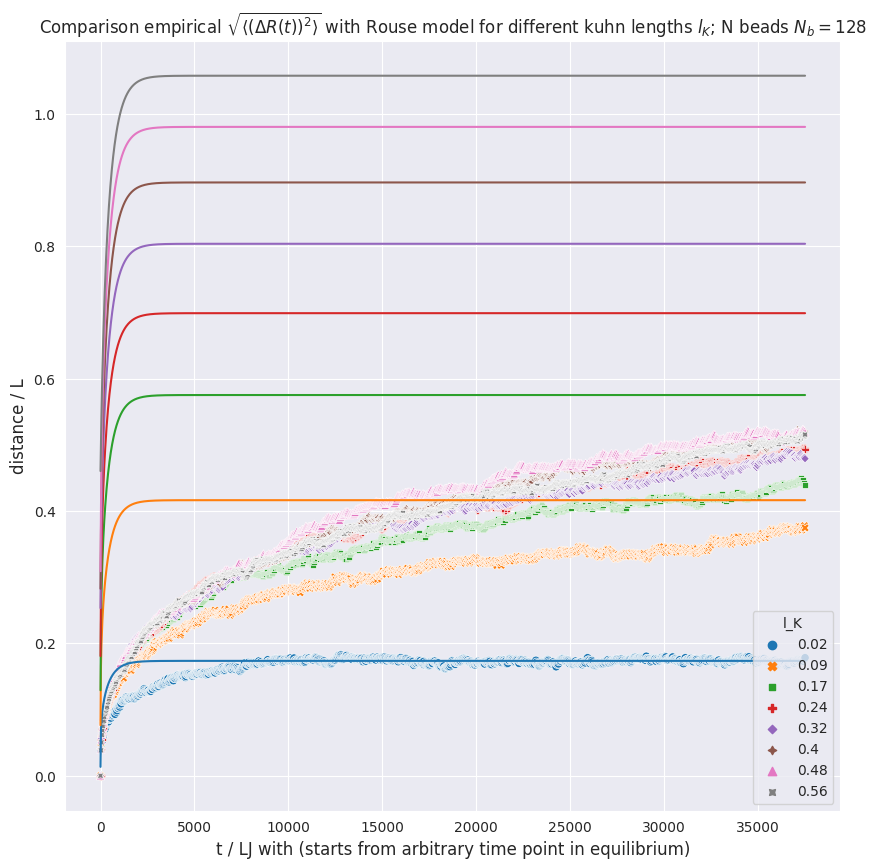
\includegraphics[width=11cm]{./4-exp-delta_R-rouse_anal.png}
    \end{figure}
\end{frame}


\begin{frame}
    \frametitle{Experiment 2: Semi-flexible chain, vary persistence length}
    \framesubtitle{$\mean{[\Delta R(t)]^2}$ vs Rouse with $\tau_R$ as free parameter}

    \begin{figure}[h]
        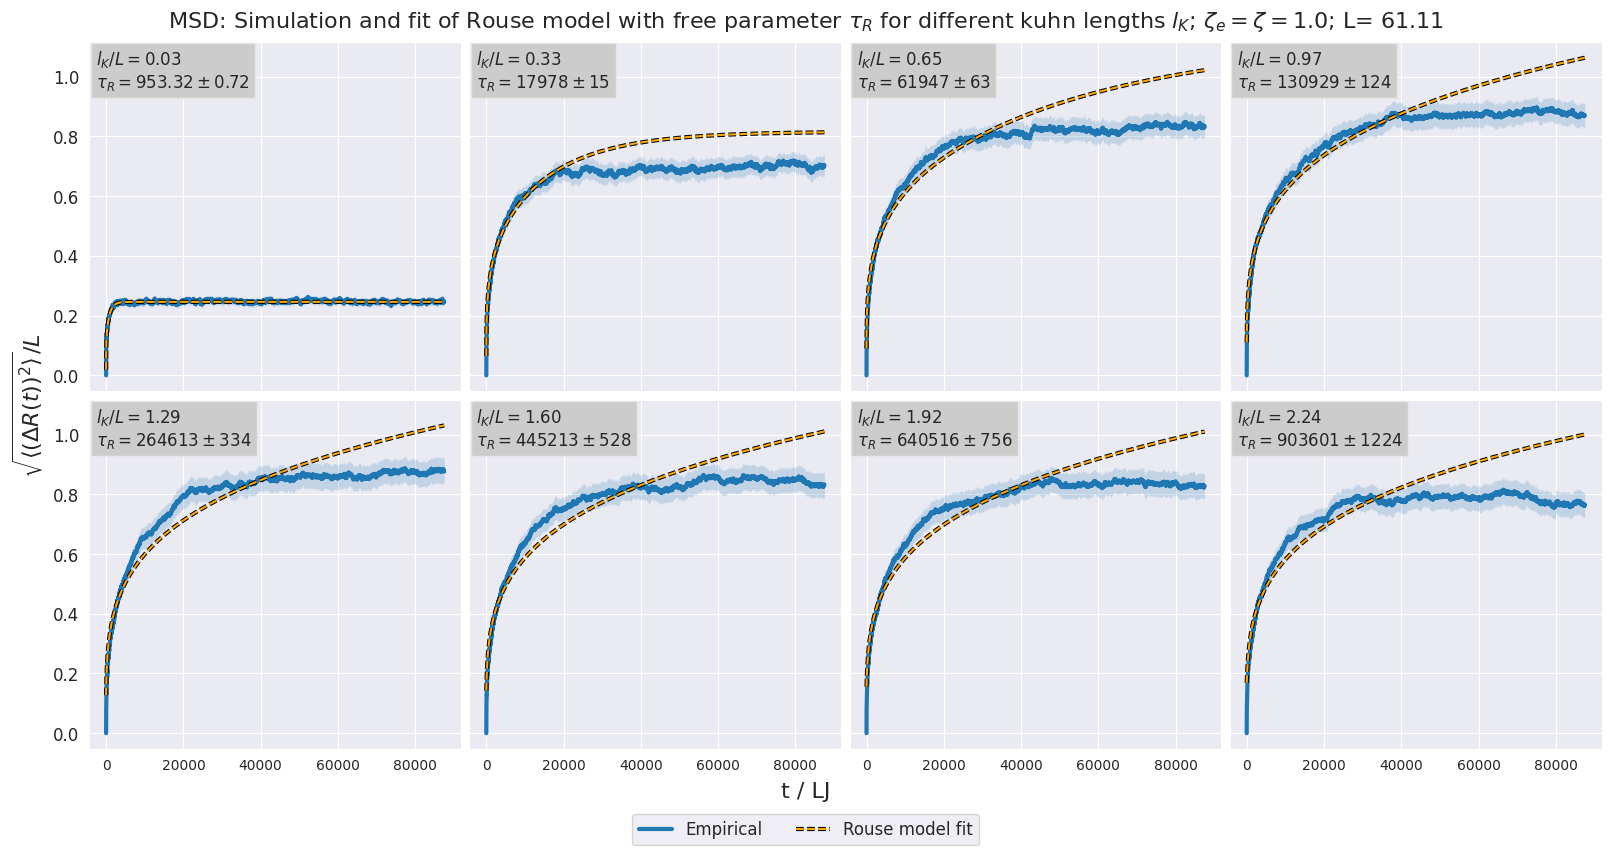
\includegraphics[width=11cm]{./4-exp-delta_R-rouse_fit.png}
    \end{figure}
\end{frame}


\begin{frame}
    \frametitle{Experiment 2: Semi-flexible chain, vary persistence length}
    \framesubtitle{Analytical and empirical $\tau_0$ vs Kuhn length}

    \begin{figure}[h]
        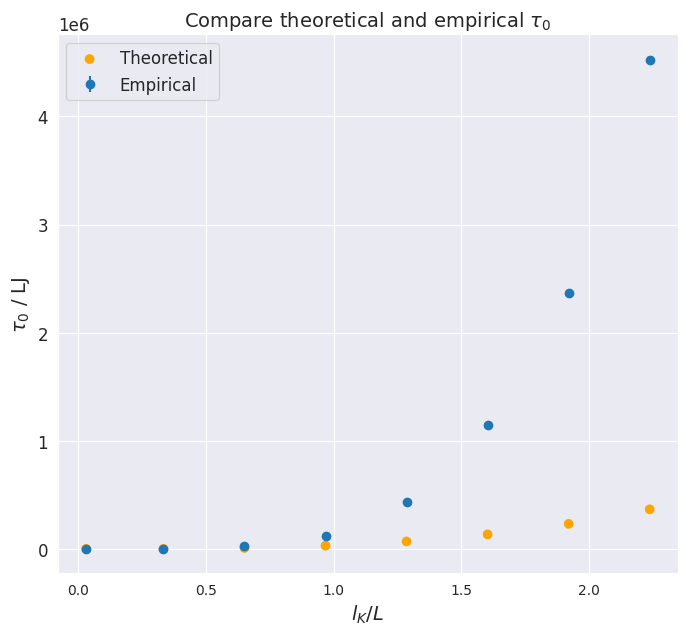
\includegraphics[width=8.5cm]{./4-exp-rouse-times.png}
    \end{figure}
\end{frame}

\begin{frame}
    \frametitle{Problems and Questions}
    \begin{enumerate}
        \item Eq. (\ref{eq:tau_R_kuhn}): Is the assumption correct? 
        Intuitively: $\zeta_{CM}=\zeta_K N_K=\zeta \frac{N_b}{N_K} N_K=\zeta N_b$, but then
        \cite[Eq. 15]{svaneborg_2020} is not proportional to $N_K^2$.
        \item Empirical $\tau_0$ are with factor $\approx 10^3$ larger then theoretical, why?
    \end{enumerate}
\end{frame}

\section{References}

\setbeamertemplate{bibliography item}{\insertbiblabel}
\begin{frame}
    \frametitle{References}
    \bibliographystyle{apalike}
    \bibliography{refs}
\end{frame}

\end{document}